\documentclass{article}
\usepackage{graphicx}
\usepackage{amsmath, amsthm, amssymb, amsfonts, amsbsy}

\begin{document}

\section{Results}
\label{sec:DL-results}


In the present section, the same datasets from the previous chapter were used. 
First it was necessary to prepare the data to be fed to the DNN.
\subsection{Data Preparation}
Each dataset was first filtered using the same filter as phy: a forwards-backwards Butterworth filter of order 3 with cutoff frequency set to 500Hz.

Each example was defined to be the array of time windows of 100 samples for each of the 127 channels in the probe. Therefore, the input data has 12700 dimensions. However, due to constraints on the available hardware, not all windows were used. Each window is shifted by 5 samples from the previous one, i.e., the first example are the 127 time windows with $t \in [ 0 , 99]$ and the second example are the 127 time windows when $t \in [ 5, 104]$. Furthermore, only samples in $t \in [1000000,2000000]$ were utilized. This yields, at this stage, 199980 examples per dataset

The windows whose central sample was closer to the Juxta Times were labeled as "1" (positive examples). Otherwise they were labeled as "0" (negative examples). The label "1" should be interpreted as "contains a spike from the juxta cell" and "0" as "doesn't contain a juxta spike". It is possible that a spike from the juxta cell be partially contained in the window of another spike from the juxta cell. However this situation is highly unlikely since for that to happen it would mean that the two spike were separated by less that 50 samples, corresponding to 1.67 ms which is less than the refractory period of cells under consideration.

This input data was split in two set: the training set (TS), with which the DNN will train, and the validation set (VS), where the resulting trained DNN is tested. The TS held 70\% of the input data (139986 examples) and VS held the remaining 30\% (59994 examples)

In table \ref{table:summary-beforeUS} is result of this splitting.
\begin{table}[htbp]
\begin{center}
\begin{tabular}{r|cc|cc|cc}
\multicolumn{1}{l|}{} & \multicolumn{ 2}{c|}{Input Data} & \multicolumn{ 2}{c|}{Training Set} & \multicolumn{ 2}{c}{Validation Set} \\ \hline
cell ID & No. of “1”  & Fraction & No. of “1”  & Fraction & No. of “1” & Fraction \\ \hline
8213 & 292 & 0.15\% & 202 & 0.14\% & 90 & 0.15\% \\ 
936 & 127 & 0.06\% & 83 & 0.06\% & 44 & 0.07\% \\ 
939 & 298 & 0.15\% & 207 & 0.15\% & 91 & 0.15\% \\ 
945 & 14 & 0.01\% & 9 & 0.01\% & 5 & 0.01\% \\ 
997 & 38 & 0.02\% & 29 & 0.02\% & 9 & 0.02\% \\ 
\end{tabular}
\end{center}
\caption{In this table are presented, for each recording, the number of examples labeled as "1" and its fraction in the Input Data, and separated in the Training Set and Validation Set. The total number of examples in the Input Data, Training Set and Validation Set are 199980, 139986 and 59994, respectively}
\label{table:summary-beforeUS}
\end{table}

As can be seen in in Table \ref{table:summary-beforeUS}, all recordings reveal a very large unbalance: there are always many more examples belonging to the class "0". In these situations, the most likely scenario is the convergence of the DNN to a trivial solution where it outputs "0" regardless of the input, yielding an accuracy equal to the fraction of examples labeled as "0".

To address this problem, it was necessary to perform upsampling: the positive examples were repeated by the same factor in both the TS and the VS. The upsampling factor was determined so that the positive examples represent around 30\% of the total number of examples in both the TS and the VS.

The results of the operation are presented in table 

\begin{table}[htbp]
\begin{center}
\begin{tabular}{c|ccc|ccc}

\multicolumn{1}{l|}{} & \multicolumn{ 3}{c|}{Training Set} & \multicolumn{ 3}{c}{Validation Set} \\ \hline
cell ID & No. of examples & No. of 1 & Fraction & No. of examples & No. of “1” & Fraction  \\ \hline
8213 & 195334 & 55550 & 28.4\% & 84654 & 24750 & 29.2\% \\ 
936 & 192276 & 52373 & 27.2\% & 87714 & 27764 & 31.7\% \\ 
939 & 195669 & 55890 & 28.6\% & 84473 & 24570 & 29.1\% \\ 
945 & 191412 & 51435 & 26.9\% & 88564 & 28575 & 32.3\% \\ 
997 & 201060 & 61103 & 30.4\% & 78948 & 18963 & 24.0\% \\ 
\end{tabular}
\end{center}
\caption{In this table are presented the details of the Training Set and Validation Set after upsampling was performed. }
\label{table:summary-afterUS}
\end{table}

This procedure artificially increases the size of datasets. However the resulting sizes are relatively close to each other and therefore DNNs trained with all the TS can be compared fairly.

\subsection{Basic Model}
In this project, we planned to study how a  feed-forward deep Neural Network performs as a spike detection for neural data. In the context of machine learning this is a binary classification problem.

It was necessary to define the basic architecture of the DNN. First and foremost, the dimension of the input layer was set to 12700 and the output layer should have only one neuron.
Usually the number of adjustable parameters in a DNN should be of the same order of magnitude of the number of examples to be used and therefore the following layer had to be much smaller. In fact, to follow this rule, the second layer should have around 15 neurons. This would be 800-fold compression which seemed excessive. Therefore, it was necessary to compromise. The second layer was define with 200 neurons. Comparatively the size of the following layer had very little influence and for that reason it was decided not to compress any further and set the dimension of layer 3 and 4 to have 200 neurons as well. 

Following the results of REFERENCE  Xavier Glorot, Antoine Bordes and Yoshua Bengio (2011) Rectified Linear Units (RELU) were should as the activation function, which should result in faster learning and weaker dependence on the initial conditions. For the last layer a sigmoid activation function was used, since the problem under consideration is of binary classification.

As for the loss function, cross entropy was chosen given its characteristic fast converge when the a activation function of the output neuron is a sigmoid.

The training algorithm was chosen to be AdaGrad.
Regarding the regularization method, the L1-norm was utilized as well as dropout with 0.2 probability parameter.

This defines the basic model of DNN that was utilized: it was a fully-connected feed-forward DNN with:
\begin{itemize}
\item $n_l$ = 5
\item $S_1 = 12700, S_2=S_3=S_4 = 200, S_5=1$
\item ReLU as activation function for hidden units and Sigmoid for the output neuron
\item Adagard as the training algorithm
\item Cross-entropy for loss function
\item L1-Regularizer along with dropout
\end{itemize}

\subsection{Optimal Hyperparameters}
\label{subsec:hyperparameters}

When defining the model to be trained some choices must be made, and there aren't exact ways of making those choices. Some are relatively straight-forward as some of the ones in the previous section. However, there are some parameter that are not as easy to set and therefore we're forced to study their influence on the performance of the DNN.

At this point, we still have to define:
\begin{itemize}
\item The size of the batch used by AdaGrad
\item The "standard" learning rate
\item The weight decay
\item The initialization method
\end{itemize}

First, the batch size was set to 10000, to be as large as the computer memory could handle.

Using the recording 939, the basic DNN was trained with different sets of parameters. 

To study the weight decay, the learning rate was fixed at $\eta = 0.001$ and LeCun Uniform was used. The results are in figures \ref{fig:study-weightdecays} and \ref{fig:study-weightdecays-zoomed}

\begin{figure}[H]
	\centering
	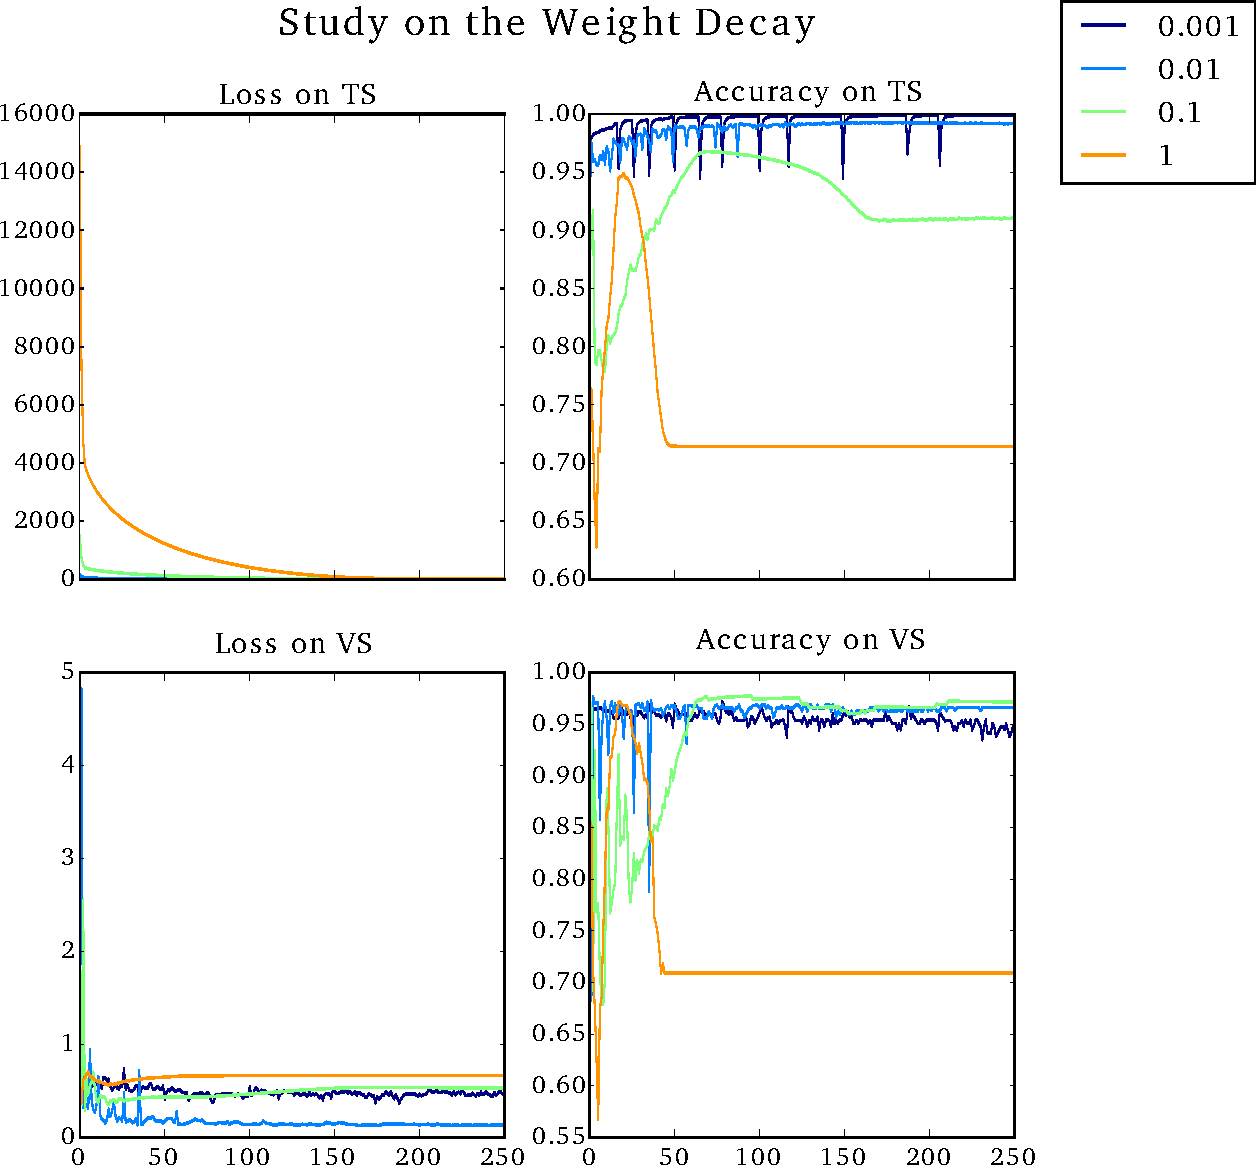
\includegraphics[width=\linewidth]{study_on_weight_decays_v2.pdf}
	\caption{Study on weight decay. Loss function and accuracies in the training set and in the validation set. LeCun uniform was used and the Learning Rate was set to $\eta = 0.001$.
}
\label{fig:study-weightdecays}
\end{figure}

\begin{figure}[H]
	\centering
	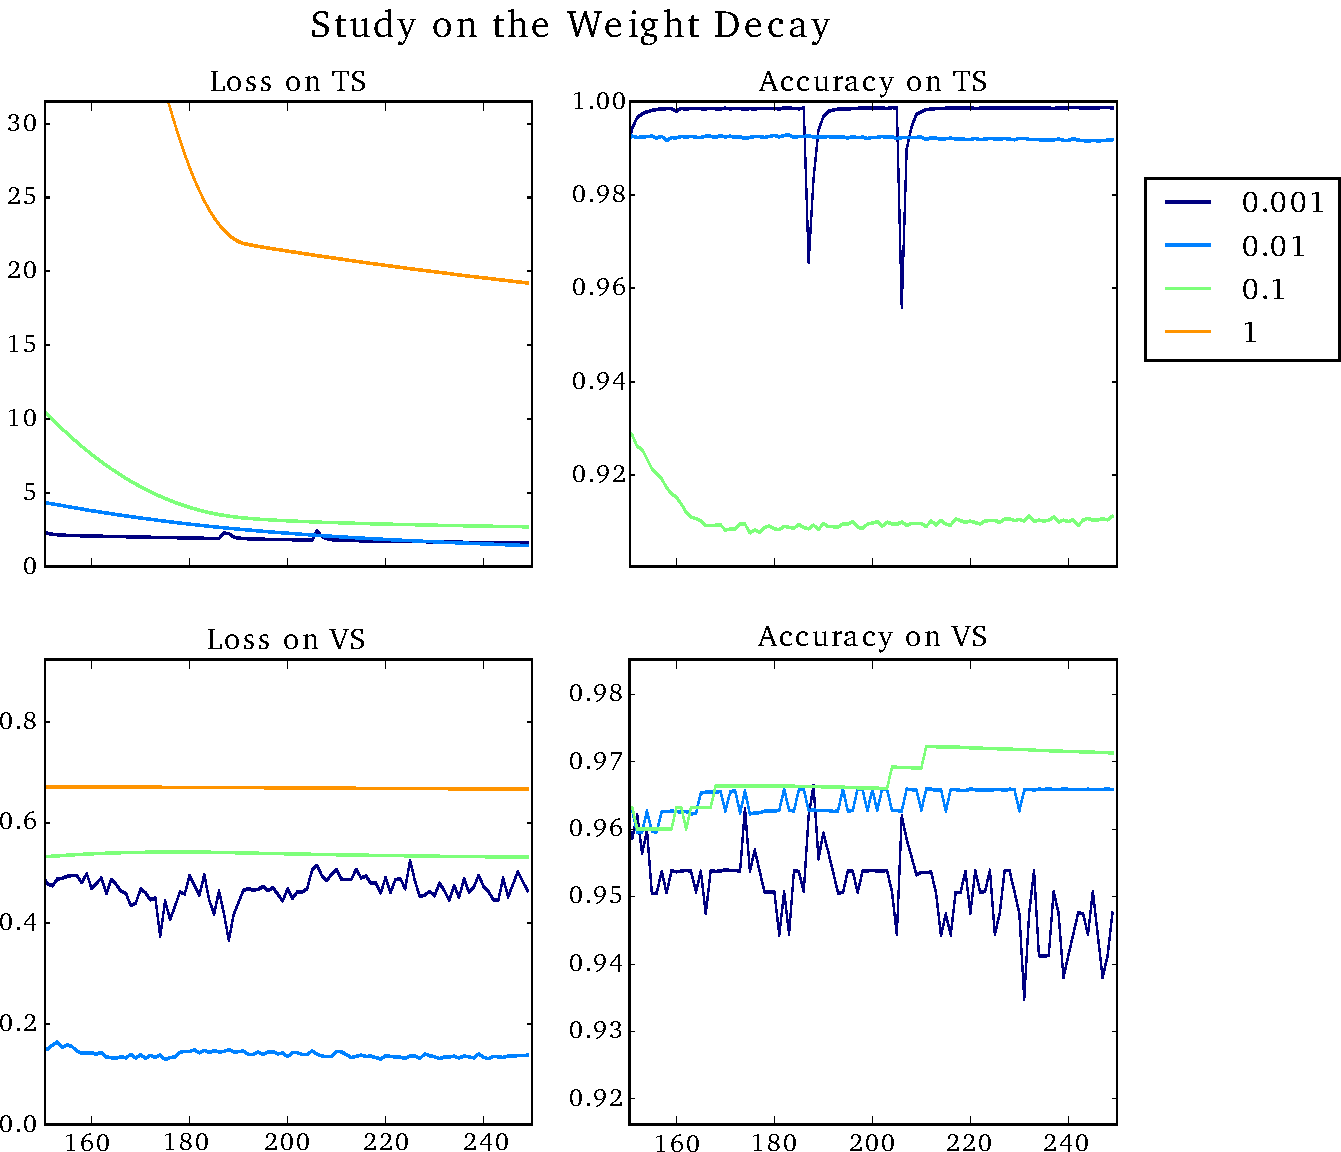
\includegraphics[width=\linewidth]{study_on_weight_decays_zoomed_v2.pdf}
	\caption{Study on weight decay - zoomed. Loss function and accuracies in the training set and in the validation set. LeCun uniform was used and the Learning Rate was set to $\eta = 0.001$.
}
\label{fig:study-weightdecays-zoomed}
\end{figure}


To study the initialization method, the learning rate was fixed at $\eta = 0.001$ and the weight decay set to $\lambda = 0.01$. The Initialization methods considered were: LeCun Uniform, He Uniform, Glorot Uniform and Uniform. The results are in figure \ref{fig:study-InitMethods} and \ref{fig:study-InitMethods-zoomed}
\begin{figure}[H]
	\centering
	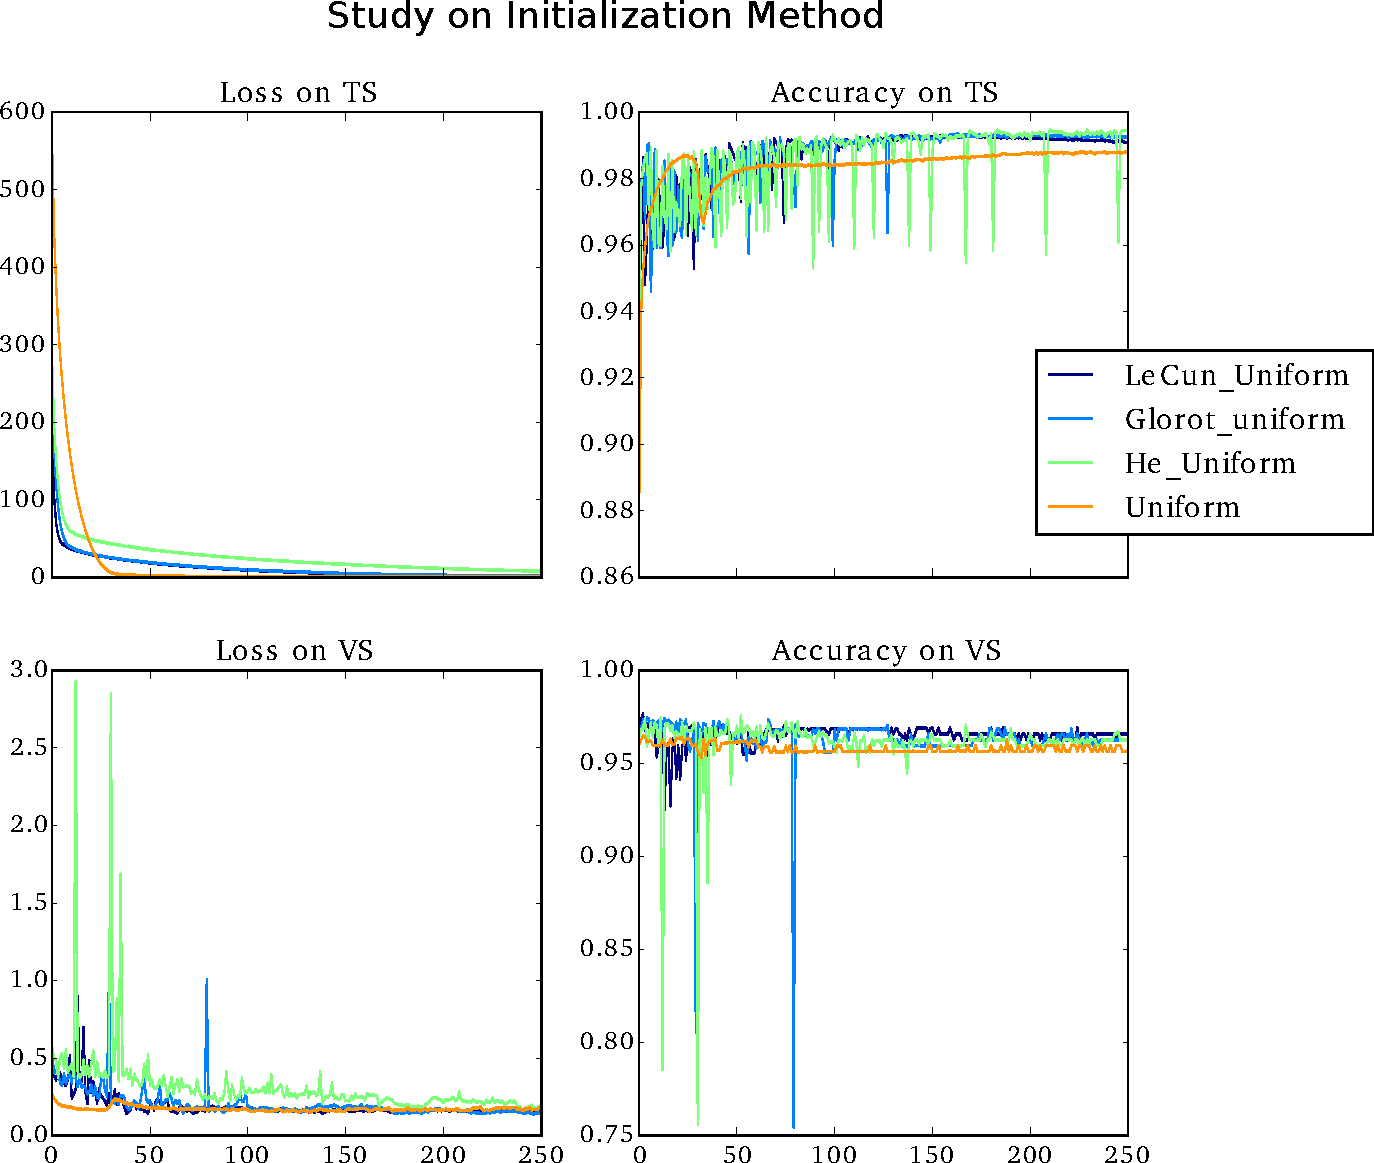
\includegraphics[width=\linewidth]{study_on_initialization_method_v2.pdf}
	\caption{Study on Initialization Methods- zoomed. Loss function and accuracies in the training set and in the validation set.The weight decay was fixed at $\lambda = 0.01$ and the Learning Rate was set to $\eta = 0.001$.
}
\label{fig:study-InitMethods}
\end{figure}

\begin{figure}[H]
	\centering
	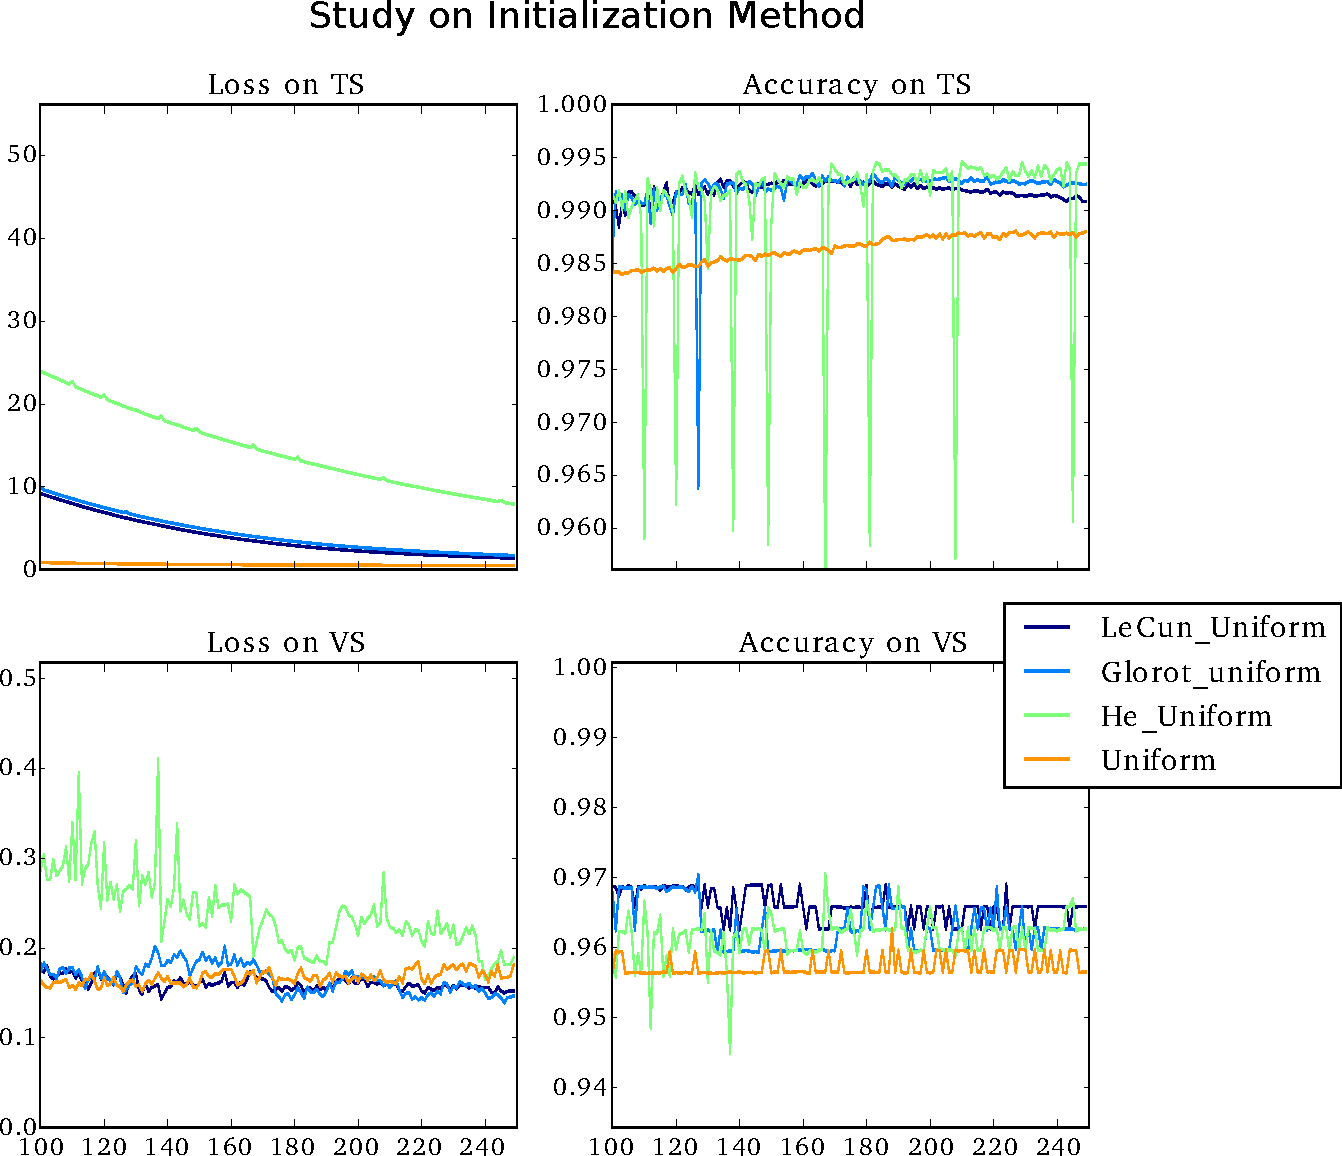
\includegraphics[width=\linewidth]{study_on_initialization_method_zoomed_v2.pdf}
	\caption{Study on Initialization Methods- zoomed. Loss function and accuracies in the training set and in the validation set.The weight decay was fixed at $\lambda = 0.01$ and the Learning Rate was set to $\eta = 0.001$.
}
\label{fig:study-InitMethods-zoomed}
\end{figure}

To study how sensitive this model was to initial conditions, different seeds for the pseudorandom generator were set. The learning rate was set to 0.001, the weight decay to $\lambda = 0.01$, and the initialization method used was LeCun Uniform. The results are in figure \ref{fig:study-seeds}

\begin{figure}[H]
	\centering
	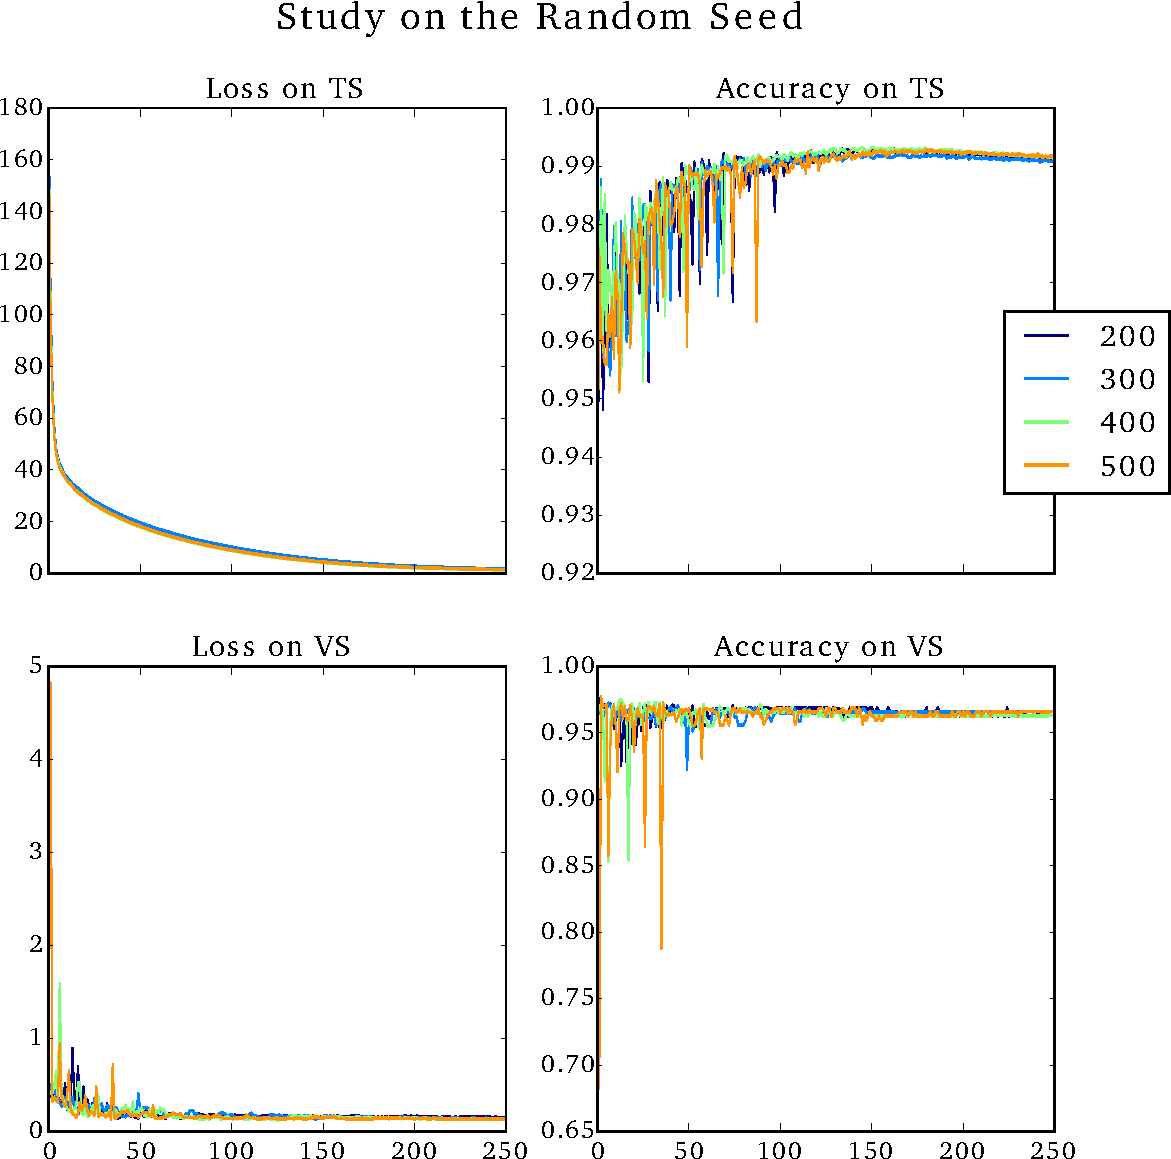
\includegraphics[width=\linewidth]{study_on_random_seed_v2.pdf}
	\caption{Study on Different Initialization. Loss function and accuracies in the training set and in the validation set.The weight decay was fixed at $\lambda = 0.01$ and the Learning Rate was set to $\eta = 0.001$ and the initialization method was LeCun Uniform.
}
\label{fig:study-seeds}
\end{figure}


To study the learning rate, the weight decay was set to $\lambda = 0.01$ and the initialization method was LeCun Uniform. The learning rate was set to 0.001, 0.01 and 0.1. The results are in the figure \ref{fig:study-LR} and \ref{fig:study-LR-zoomed}

\begin{figure}[H]
	\centering
	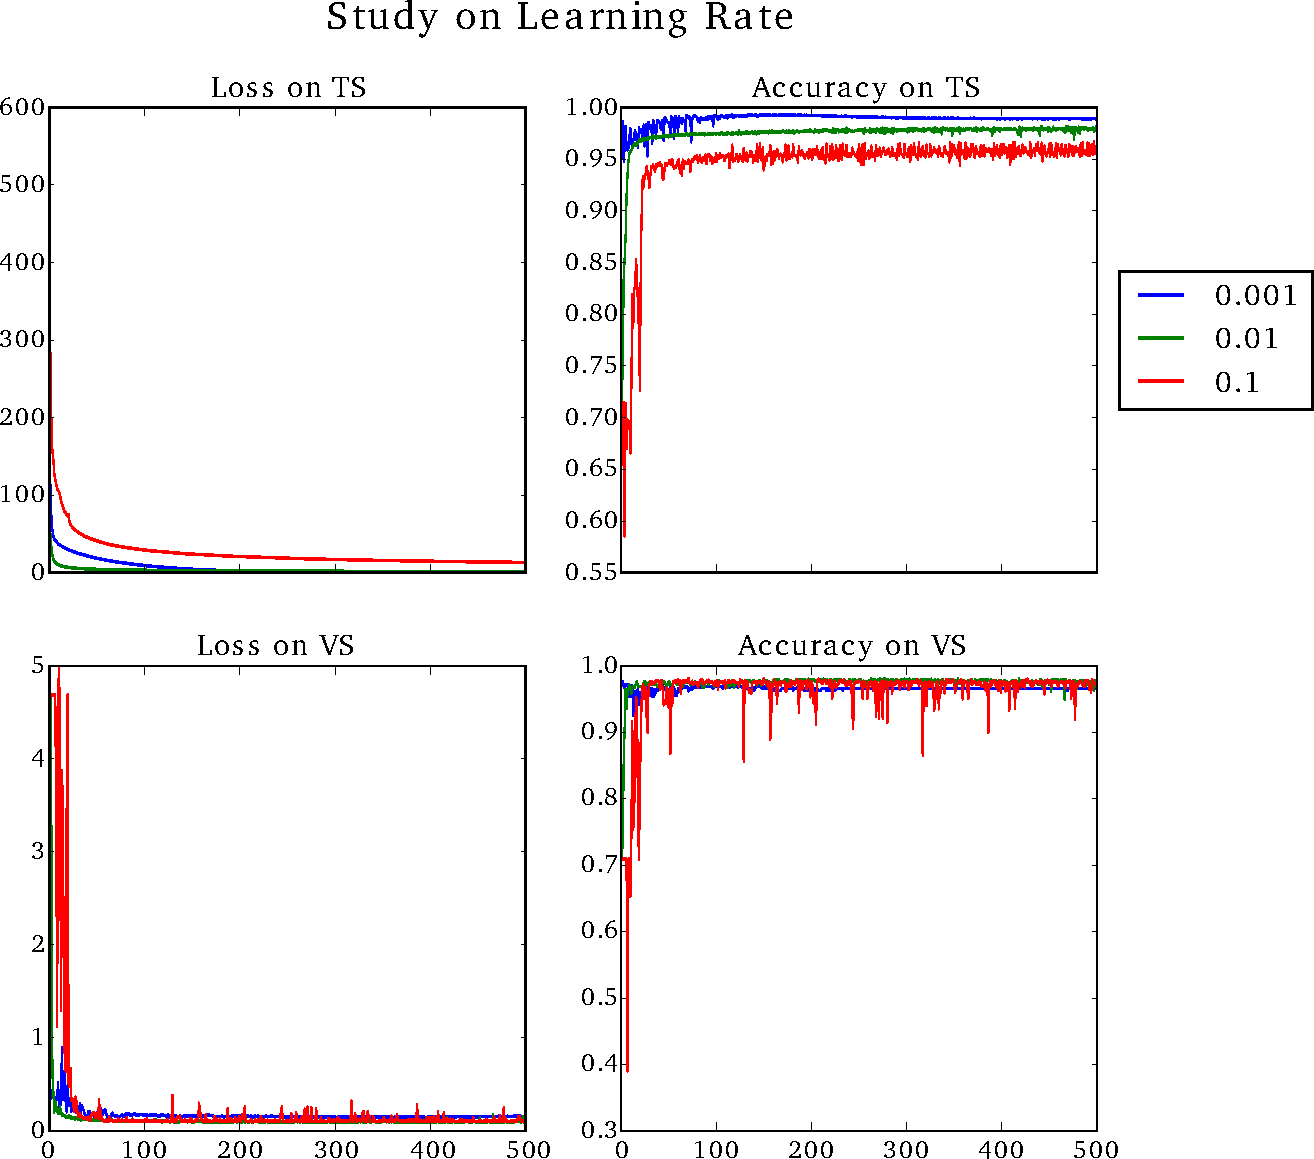
\includegraphics[width=\linewidth]{study-on-LR.pdf}
	\caption{Study on Learning Rate. Loss function and accuracies in the training set and in the validation set.The weight decay was fixed at $\lambda = 0.01$, and the initialization method was LeCun Uniform.
}
\label{fig:study-LR}
\end{figure}


\begin{figure}[H]
	\centering
	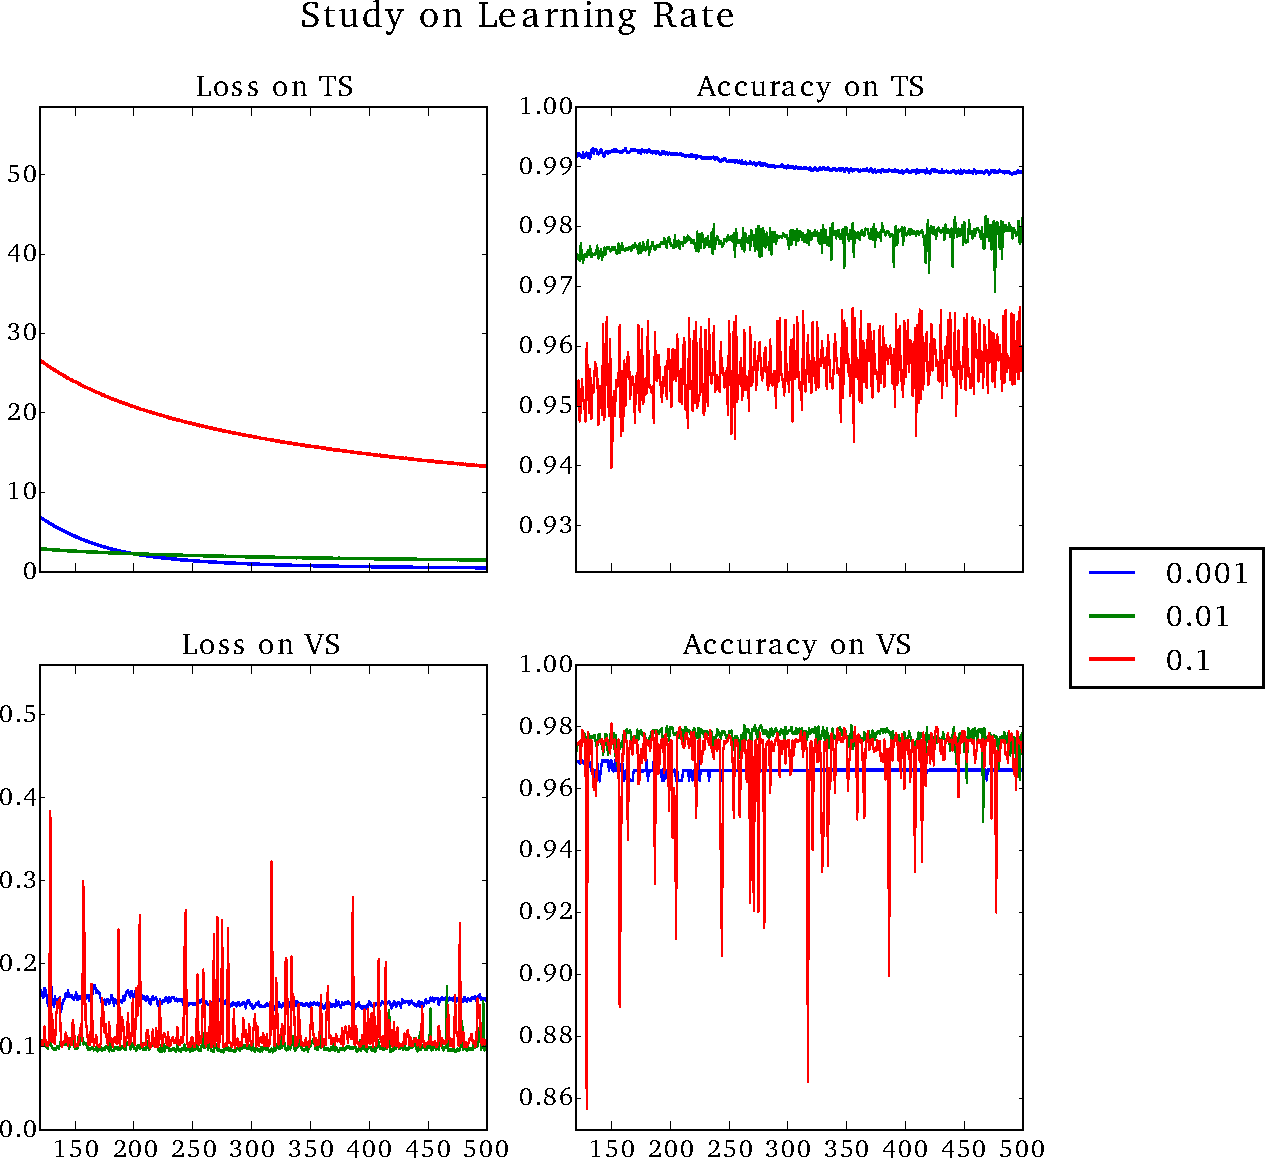
\includegraphics[width=\linewidth]{study-on-LR-zoomed-ending.pdf}
	\caption{Study on Learning Rate - zoomed. Loss function and accuracies in the training set and in the validation set.The weight decay was fixed at $\lambda = 0.01$, and the initialization method was LeCun Uniform.
}
\label{fig:study-LR-zoomed}
\end{figure}

The best value for the weight decay seemed to be $\lambda = 0.01$, since higher values led the network to converge onto bad solutions even in the training set. With $\lambda = 0.001$ the training led to overfitting of the TS and the performance on the VS begins to drop.

LeCun Uniform turned out to be the best initialization method. All of the methods yield good results and are hardly distinguishable when the number of epochs is large. However LeCun Uniform gives gives the best values of accuracy in the VS and leads to a much more stable training without big oscillations on the accurary on the VS.

From figure \ref{fig:study-seeds} it can be seen that the network is not sensitive to variations in the actual initial values of the parameter, since the performance parameters varies very little after around 50 epochs.

Regarding the learning rate, the performance in the training set is best the $\eta = 0.001$ even though it starts to get worse after around 80 epochs. On the validation set this value seems to yield the most stable convergence but the one with the worst performance. However, for the rest of this chapter this was the value chosen for the learning rate.

The depth of the network was also tested, by comparing the performance of DNNs with two, three and four hidden layers. To keep the number of adjustable parameter approximately the same these networks had the following architecture:
12700-205-205-1, 12700-200-200-200-1 and 12700-195-195-195-195-1, with 2646551, 2620801 and 2591551 parameters, respectively. The results are in figure \ref{fig:study-depth}

All networks achieved the same performance in the validation set. However, the networks with three hidden layers seems to have a more stable convergence and for that reason was the one adopted.

\begin{figure}[H]
	\centering
	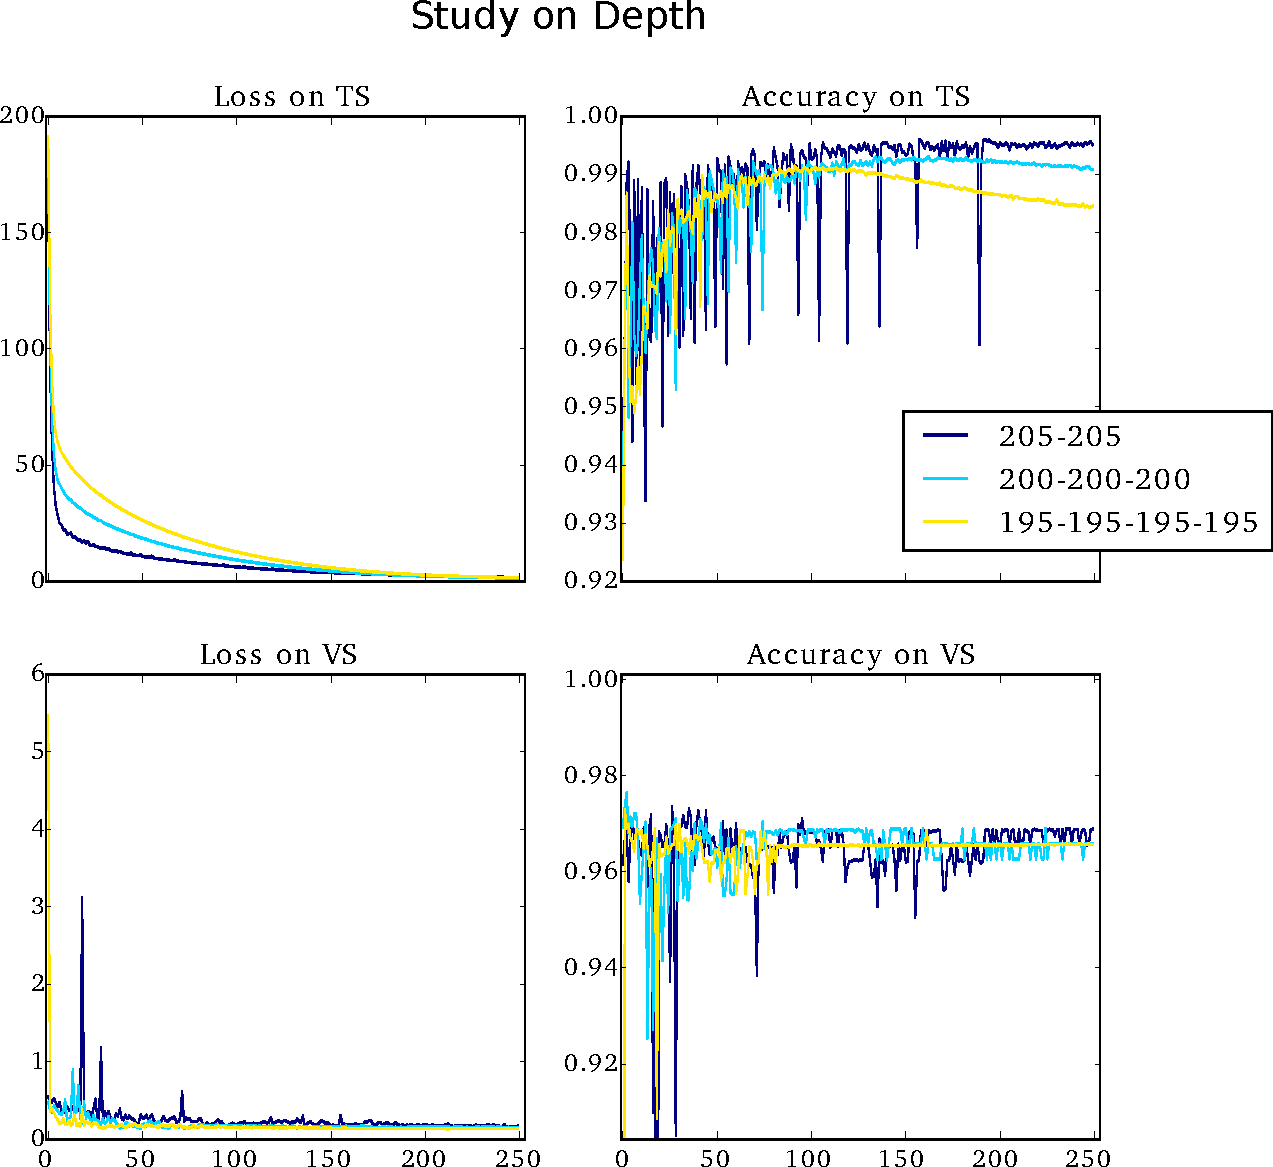
\includegraphics[width=\linewidth]{study_on_depth_v2.pdf}
	\caption{Study on Depth. Loss function and accuracies in the training set and in the validation set.The learning rate was $\eta = 0.001$, the weight decay was fixed at $\lambda = 0.01$, and the initialization method was LeCun Uniform.
}
\label{fig:study-depth}
\end{figure}

\subsection{Application to Dataset from Neto et al.}
\label{subsec:application}
The optimal hyperparameters and configurations discussed in the previous section were used in the training of the DNN with all the datasets. The performance results are in Fig. \ref{fig:study-cells} and Fig. \ref{fig:study-cells-zoomed}

\begin{figure}[H]
	\centering
	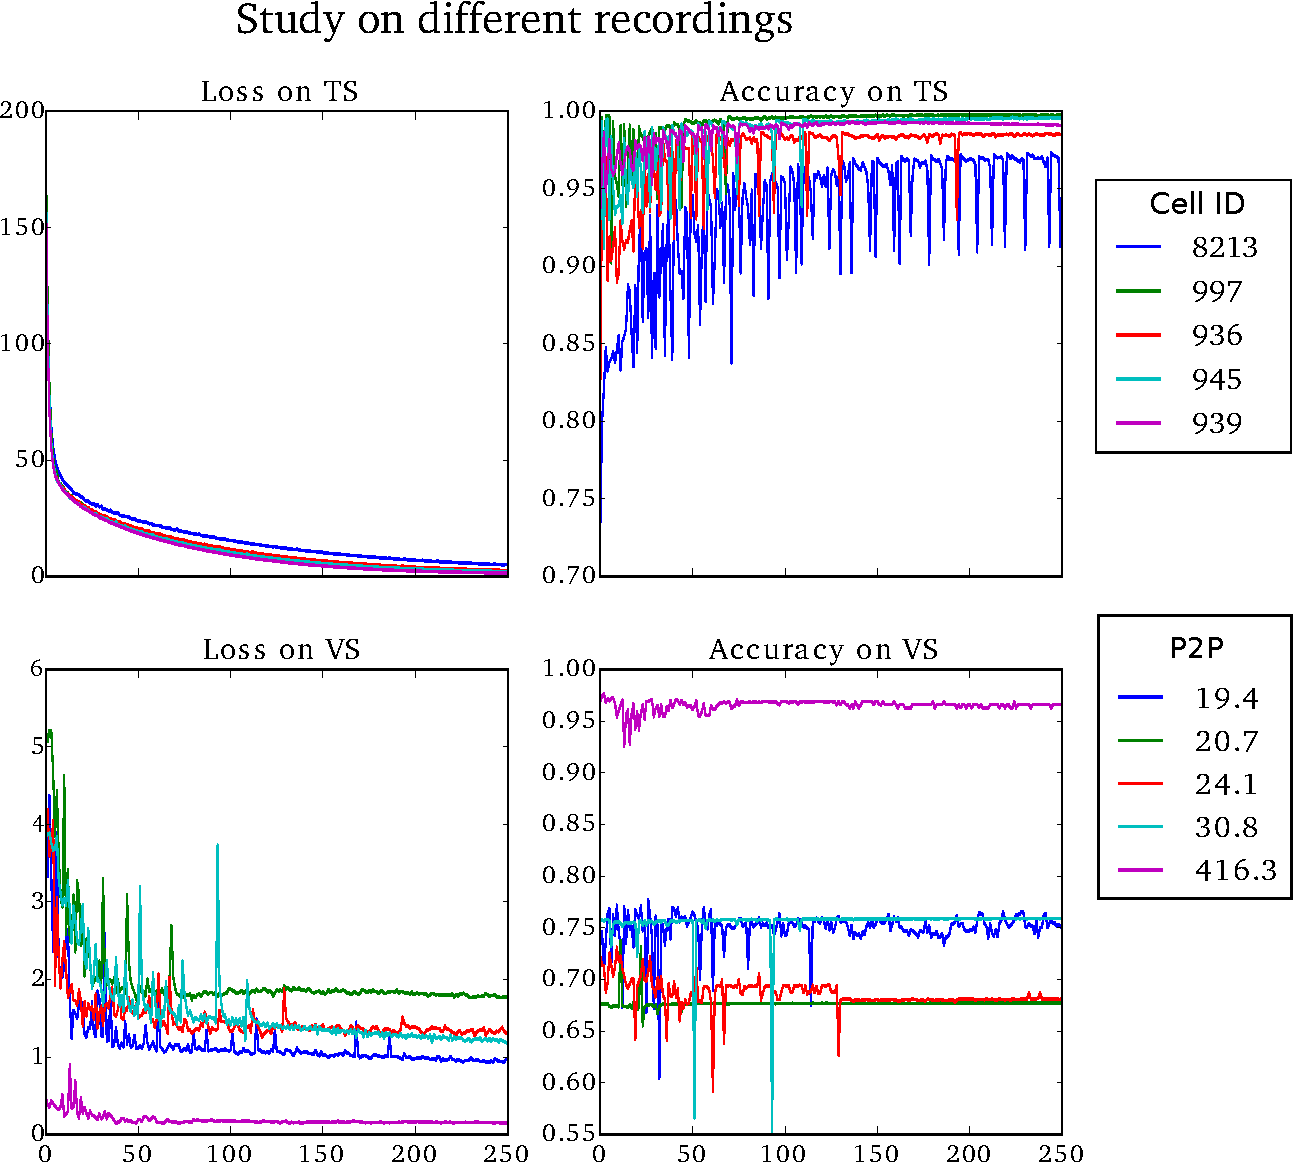
\includegraphics[width=\linewidth]{study_on_different_cells_v2.pdf}
	\caption{Study on Different Recordings. Loss function and accuracies in the training set and in the validation set.The learning rate was $\eta = 0.001$, the weight decay was fixed at $\lambda = 0.01$, and the initialization method was LeCun Uniform. On the legend on the top is the Cell ID and on the legend on the bottom are the P2P amplitude.
}
\label{fig:study-cells}
\end{figure}

\begin{figure}[H]
	\centering
	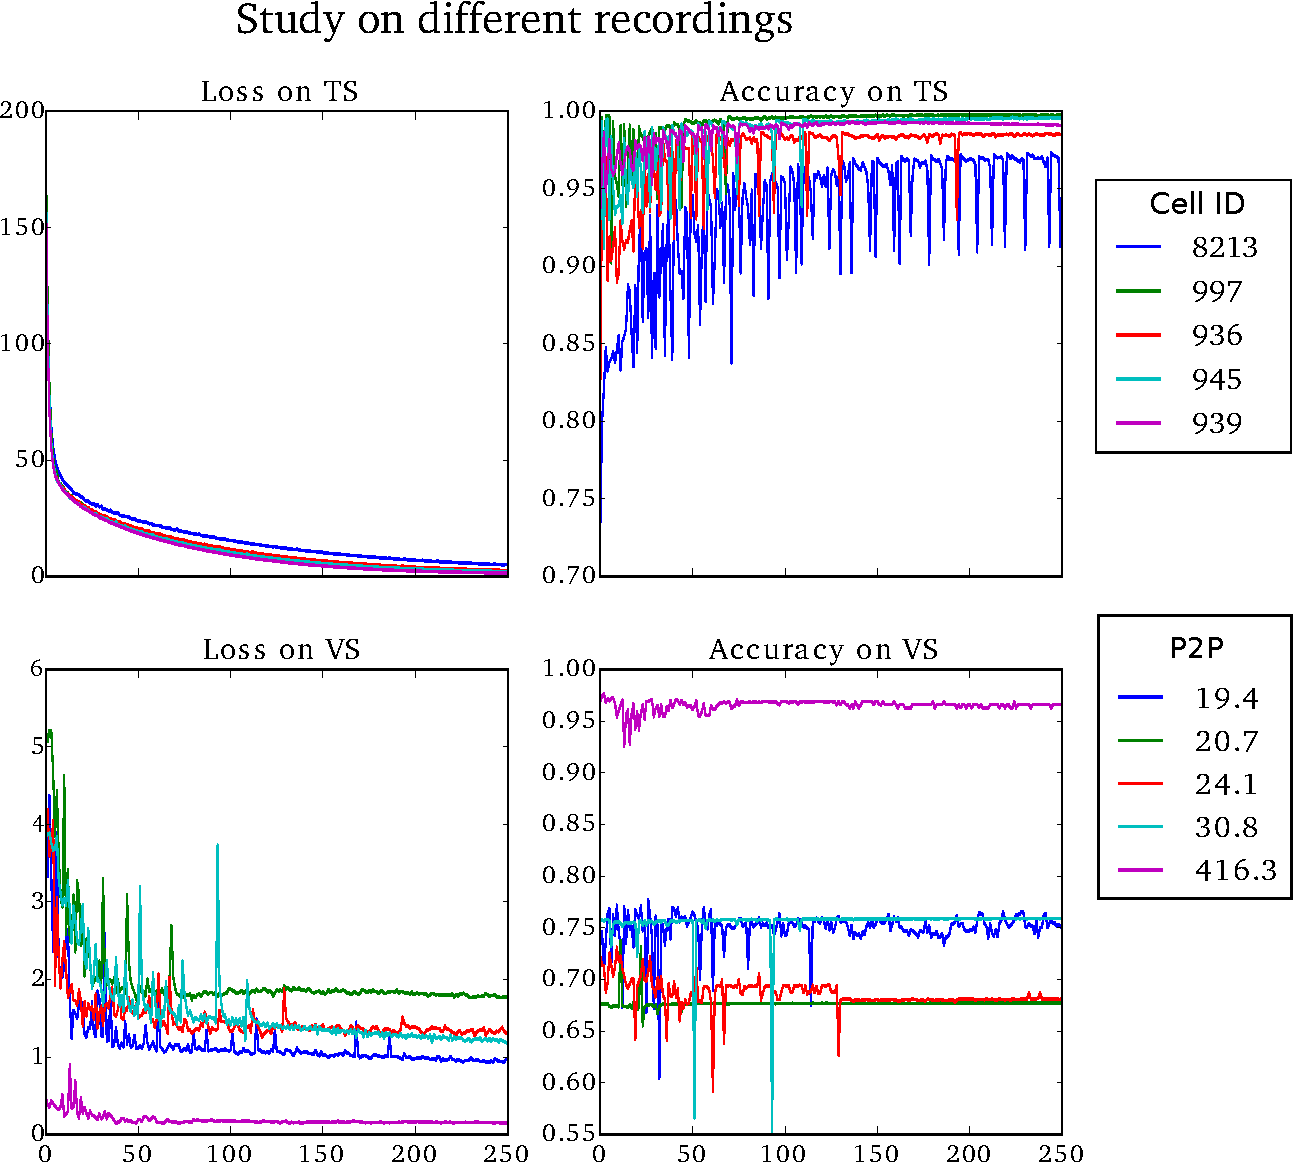
\includegraphics[width=\linewidth]{study_on_different_cells_v2.pdf}
	\caption{Study on Different Recordings. Loss function and accuracies in the training set and in the validation set.The learning rate was $\eta = 0.001$, the weight decay was fixed at $\lambda = 0.01$, and the initialization method was LeCun Uniform. On the legend on the top is the Cell ID and on the legend on the bottom are the P2P amplitude.
}
\label{fig:study-cells-zoomed}
\end{figure}
Looking at the accuracy on the training set, one can 
The figures present three different situations. On the case of the recording 939, an accuracy of around 97\% is achieve.
\end{document}